Emphatic-TD (ETD), proposed by Sutton et al. in 2015, is the most promising way to mitigate off-policy training instability. It works by estimating the transitive dependency between states (called the \emph{followon trace}) and uses that to reweight TD updates to appear on-policy.

Estimating the followon trace is very difficult. Modern ETD algorithms do this using a form of reversed TD, which makes it vulnerable to regularization bias.
\begin{center}
    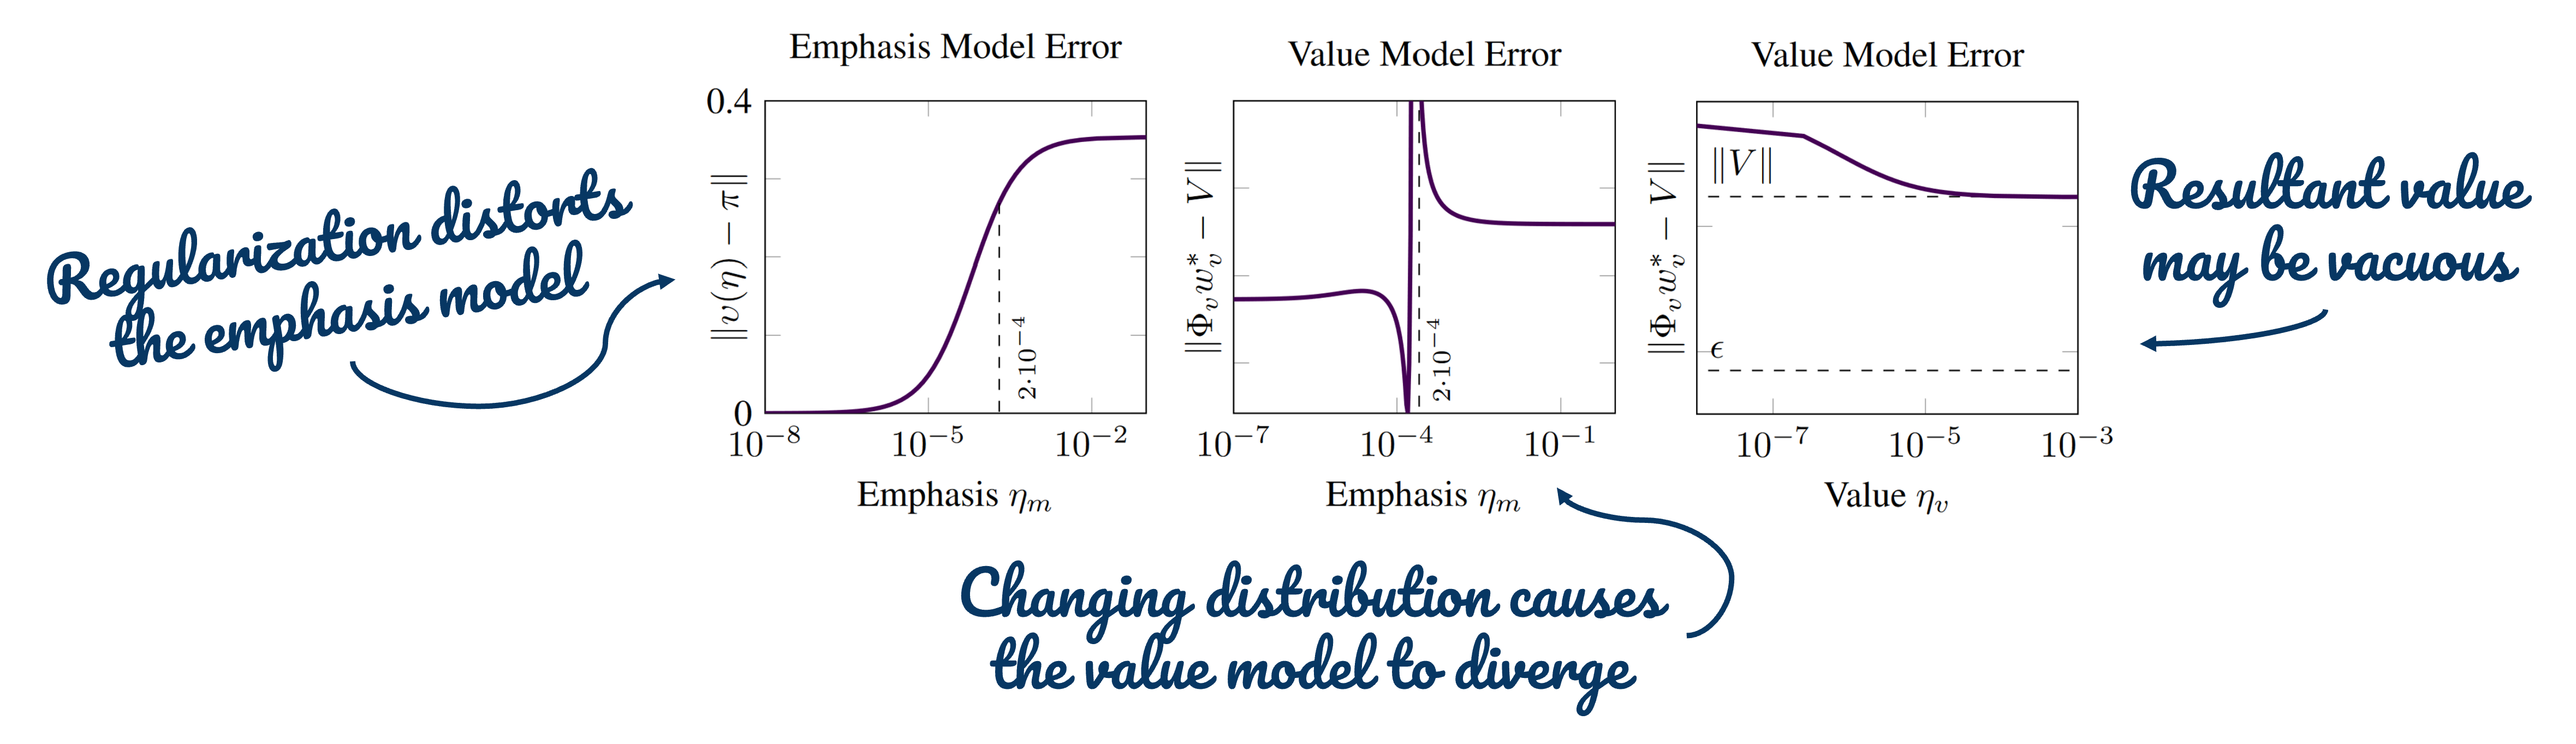
\includegraphics[scale=0.4]{parts/emphatic/emphatic.png}
\end{center}
All trained models exhibit a bump in error at similar levels of regularization, showing that this divergence is not an artifact of poor initialization.
